\documentclass[11pt]{article}
\usepackage[utf8]{inputenc}
\usepackage[T1]{fontenc}
\usepackage{lmodern}
\usepackage[margin=1in]{geometry}
\usepackage{amsmath,amssymb}
\usepackage{graphicx}
\usepackage{xcolor}
\usepackage{authblk}
\usepackage[hidelinks]{hyperref}
\usepackage{booktabs}
\usepackage{siunitx}
\usepackage[font=small,labelfont=bf]{caption}

\newcommand{\rca}{\mathrm{RCA}}
\newcommand{\I}{\mathcal{I}}
\newcommand{\N}{\mathcal{N}}

\title{\textbf{Antimicrobial resistance is a block-nested ecosystem:\\
economic-complexity structure and prediction of resistance emergence}}
\date{\today}

\begin{document}
\maketitle

\begin{abstract}
\noindent
Antimicrobial resistance (AMR) is usually monitored one pathogen--antibiotic pair at a time,
ignoring the global structure of the resistance landscape. Here we represent AMR surveillance
data as a bipartite pathogen--antibiotic network and analyse it with tools from Economic Complexity.
Using \num{394} species, \num{43} antibiotics and two decades (2004--2024) of the ATLAS/Vivli
surveillance programme, we show that the resistance network is not \emph{globally nested} like the
country--product trade network, but \emph{block-nested} like the firm--product network: global
nestedness is absent ($\N$ below a degree-preserving null), whereas an in-block nestedness
$\I^\ast/\N=7.8$ ($z=10.3$) emerges once the network is partitioned into drug-spectrum blocks. This
structure explains why the Fitness--Complexity (FC) algorithm is degenerate when applied globally,
but yields meaningful rankings within blocks: antibiotic resistance complexity correlates with the
WHO AWaRe classification ($\rho=0.6$), and pathogen fitness separates ESKAPEE from non-ESKAPEE
organisms ($p<10^{-3}$), whereas the corresponding global scores fail (fitness vs.\ WHO priority
$\rho=-0.24$, mirroring the firm--product case). Finally, projecting the bipartite network onto
either layer yields a resistance-relatedness network on which the emergence of new resistance is
predictable out of sample: a parameter-free network-exposure score anticipates which susceptible
pathogen--antibiotic pairs become resistant in a rolling-origin test over 2020--2024 (AUC $0.71$,
$p<0.005$), while resistance prevalence and proximity-to-threshold carry no information after a
comparative-advantage binarization. AMR is thus
a modular, locally-nested ecosystem in which resistance spreads by predictable local contagion.
\end{abstract}

\section{Introduction}
Antimicrobial resistance is one of the leading global health threats, associated with over a million
deaths per year. Surveillance programmes such as the Pfizer ATLAS dataset (distributed through Vivli)
record, for each bacterial isolate, the antibiotics it was tested against and whether it was
susceptible, intermediate or resistant. These data are conventionally summarised as pairwise
resistance rates: the fraction of a given species resistant to a given drug. Yet the clinical and
evolutionary meaning of resistance is relational---resistance to a broadly effective, last-line drug
is not equivalent to resistance to an already-compromised one, and the drugs a pathogen resists are
not independent draws but reflect shared mechanisms and co-selection.

The Economic Complexity (EC) framework was developed to extract exactly this kind of relational
information from bipartite networks~\cite{hidalgo2009,tacchella2012}. Applied to the country--product
export network, it uncovers a nested structure that underlies the Fitness--Complexity (FC) algorithm
and enables data-driven forecasts of economic growth. The same toolbox---bipartite projections,
relatedness networks, fitness and complexity---has since been applied to jobs and skills~\cite{aufiero2024},
to chess openings~\cite{demarzo2023chess}, and, crucially for us, to firms~\cite{laudati2023}, where
the network was found to be \emph{block-nested} rather than globally nested, so that FC must be applied
\emph{within} locally-nested blocks.

Here we ask whether the AMR pathogen--antibiotic network can be understood through the same lens, and
whether its structure makes resistance emergence predictable. We find that AMR behaves like the firm
ecosystem: it is block-nested, its blocks correspond to antibiotic spectrum, within-block FC scores
agree with independent WHO expert classifications, and a network-exposure predictor forecasts new
resistance out of sample. We report the results first, then discuss implications and methods.

\section{Results}

\subsection{From resistance rates to a resistance network}
The starting point is a simple table: for every bacterial species and every antibiotic, what
fraction of the tested samples were resistant. We build this table from two decades of surveillance
(\num{394} species, \num{43} antibiotics, 2004--2024), keeping only well-sampled cases with at least
\num{30} tested isolates (\num{11507} such cases). The raw resistance fraction $r_{pa}$
(Fig.~\ref{fig:bin}a) is, however, a misleading quantity to compare across the table, because it is
dominated by two trivial effects: some drugs (ampicillin, penicillin) are old and beaten by almost
everything, and some species resist almost everything. A high number can therefore mean either a
genuinely notable resistance or simply that the drug is generally weak.

To strip out these size effects we use a measure borrowed from economics, the \emph{revealed
comparative advantage} (RCA), which asks a sharper question: does this species resist this drug
\emph{more than one would expect by chance}, given how resistant the species is overall and how
vulnerable the drug is overall? When it does---$\rca_{pa}\ge 1$---we mark an effective resistance
link (Fig.~\ref{fig:bin}b). This cutoff is not tuned for our results: on our data $\rca=1$ falls right
at the \emph{median} of the RCA distribution (median $\rca=0.99$--$1.17$ across time windows), so it
simply separates ``more resistant than typical'' from ``less''. The outcome is a clean yes/no matrix
$M_{pa}$ (Fig.~\ref{fig:bin}c), and this is the object we analyse throughout. The step matters: as we
show below, it removes exactly the confounds---how common a resistance is, and how close a species
already sits to the threshold---that would otherwise masquerade as prediction, leaving only the
genuine network signal.

\begin{figure}[t]
\centering
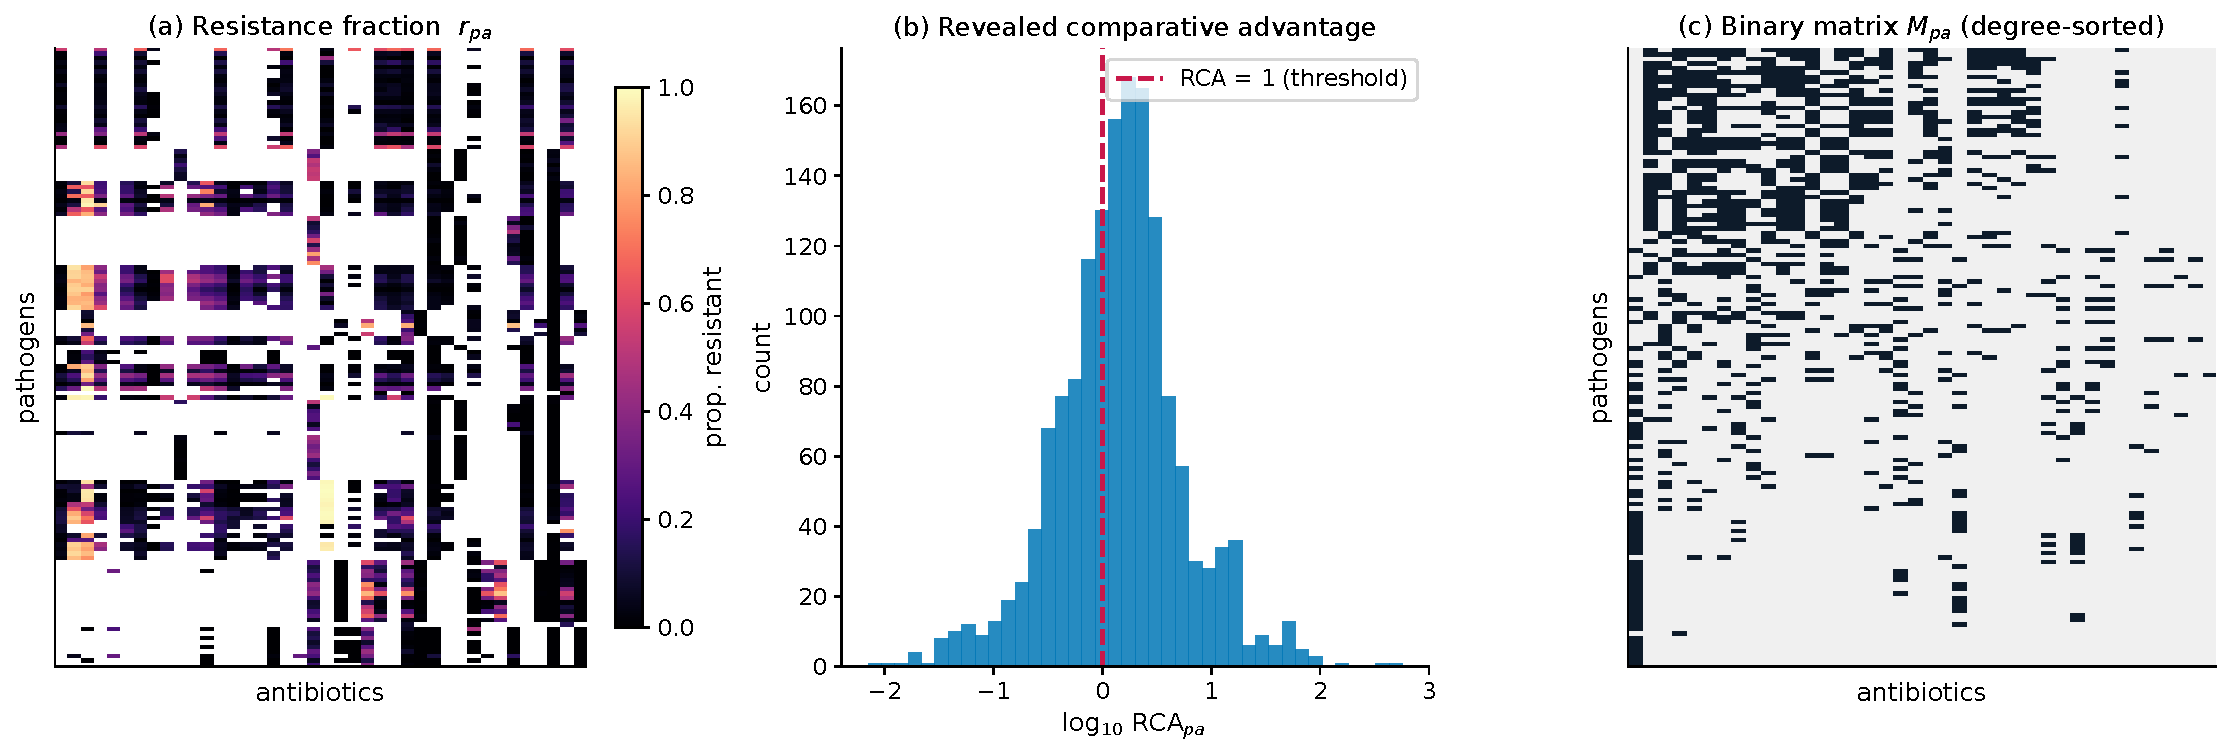
\includegraphics[width=\textwidth]{figures/fig1_binarization.pdf}
\caption{\textbf{Construction of the bipartite resistance network.}
(a) Resistance fraction $r_{pa}$ for pathogens (rows) $\times$ antibiotics (columns).
(b) Distribution of the revealed comparative advantage $\rca_{pa}$; the threshold $\rca=1$ (dashed)
defines effective resistance links. (c) Resulting binary matrix $M_{pa}$, degree-sorted.}
\label{fig:bin}
\end{figure}

\subsection{A modular landscape, not a single ladder}
The first question is how the resistance table is organised as a whole. In world trade, the analogous
country--product table is \emph{nested} like a ladder: the most developed countries export nearly
everything, less developed ones export only a subset of the same common goods, and the rare,
sophisticated products are made only at the top. If AMR worked the same way, there would be a single
ladder of ``super-resistant'' bugs at the top that beat every drug, down to specialists at the bottom.
We test this with a standard nestedness score $\N$ and its within-group version
$\I$~\cite{soleribalta2018,laudati2023}.

AMR does \emph{not} form a single ladder. Measured globally, its nestedness is negligible
($\N=0.05$)---in fact slightly \emph{below} what one would get by chance ($z=-4.3$). But this is not
disorder: when we first split the drugs and bugs into groups (by spectral co-clustering) and measure
nestedness \emph{inside} each group, it jumps to $\I^\ast=0.39$, almost eight times the global value
($\I^\ast/\N=7.8$; far above chance, $z=10.3$; Fig.~\ref{fig:block}b). In other words, the resistance
landscape is \emph{modular}: it is made of several separate ladders rather than one. This is exactly
the pattern Ref.~\cite{laudati2023} found for companies (ratio $\approx 12$) and the opposite of the
one for countries ($\approx 1.02$)---AMR sits firmly on the company-like, modular side.

Reassuringly, the groups the algorithm finds are the ones a microbiologist would draw
(Fig.~\ref{fig:block}a): a large Gram-negative $\beta$-lactam block (Enterobacterales), a Gram-positive
block, a block of enterococci resisting glycopeptides (the VRE ecosystem), and an anaerobe block. So
the ladder structure is real but \emph{local}: within a single therapeutic ecosystem the bugs that
beat the rare drugs also beat the common ones, but this ordering simply does not carry across
ecosystems---a drug that is hard to resist for a Gram-negative says nothing about a Gram-positive.

\begin{figure}[t]
\centering
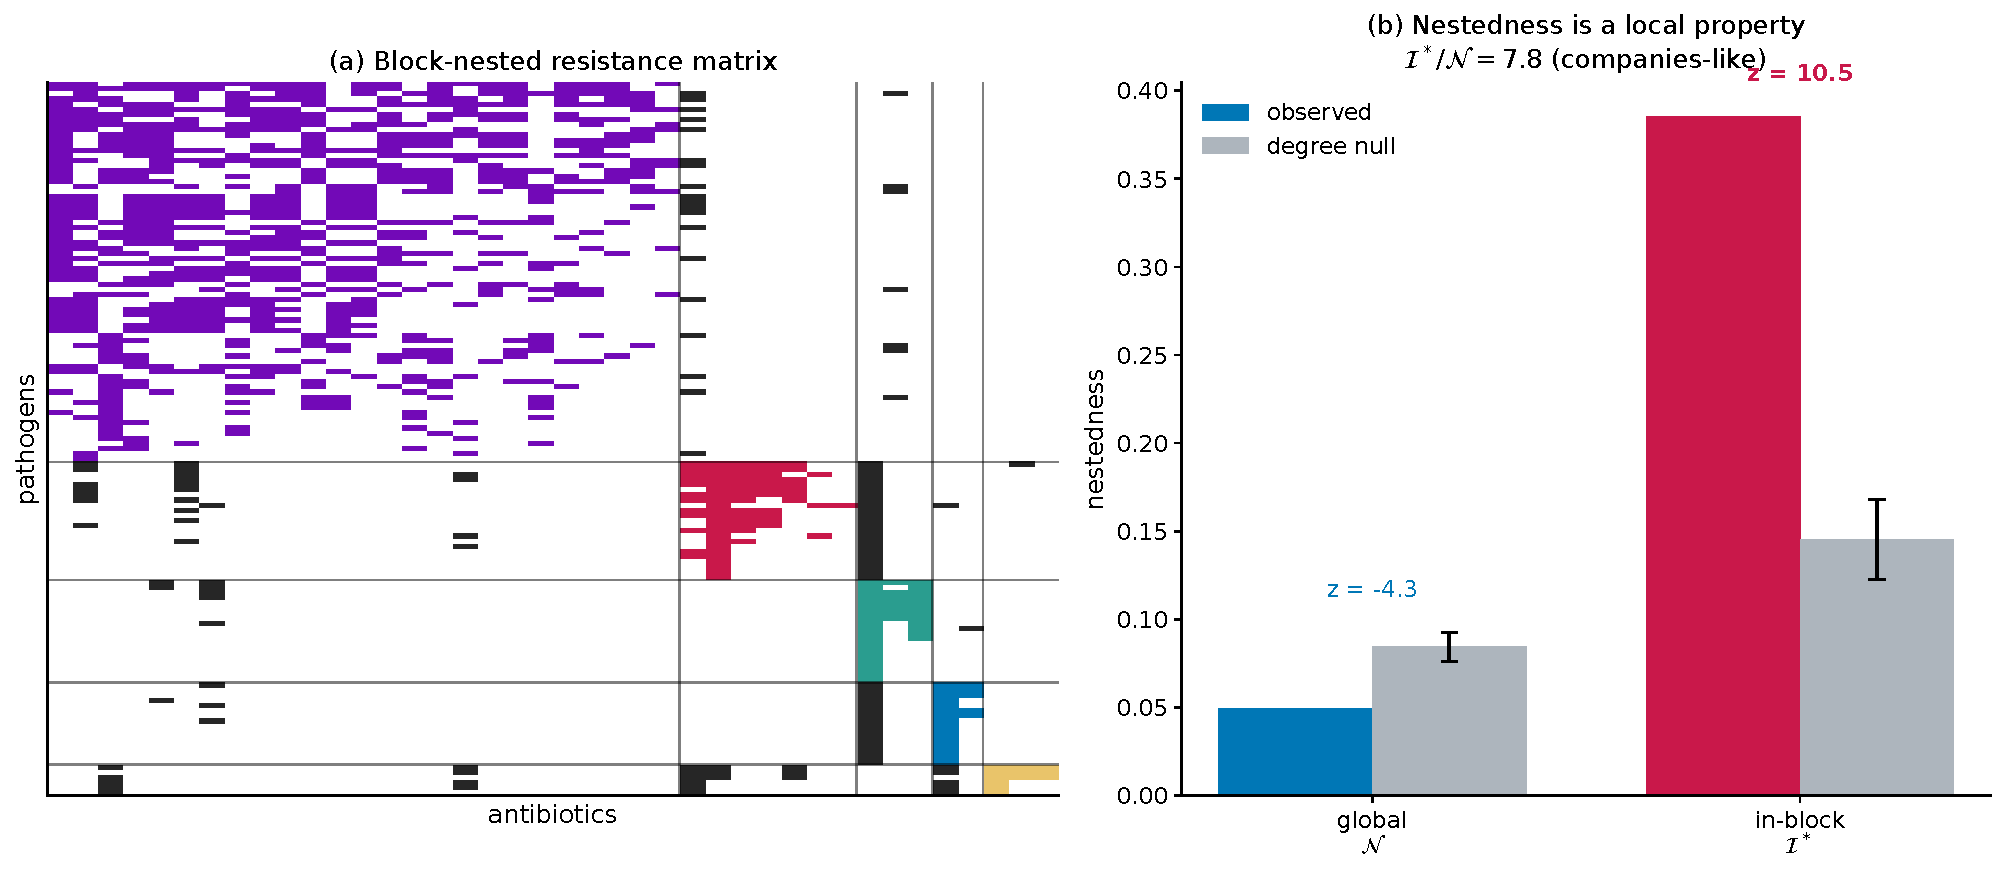
\includegraphics[width=\textwidth]{figures/fig2_blocknested.pdf}
\caption{\textbf{AMR is block-nested.}
(a) The binary resistance matrix reordered by co-clustered blocks (colours) and by degree within each
block; off-block links in dark grey. Each block is internally nested (triangular).
(b) Global nestedness $\N$ and in-block nestedness $\I^\ast$ versus a degree-preserving null.
$\N$ is below the null ($z=-4.3$) while $\I^\ast$ is far above it ($z=10.3$), giving $\I^\ast/\N=7.8$.}
\label{fig:block}
\end{figure}

\subsection{Ranking bugs and drugs, and checking it against the WHO}
Economic Complexity summarises such a table with two intuitive scores. A country's \emph{fitness} is
high if it exports many things, especially hard ones; a product's \emph{complexity} is high if only
the most capable countries make it. We compute the same two scores here~\cite{tacchella2012}, reading
a pathogen as a ``country'' that carries resistances and a drug as a ``product'': a bug's fitness is
then the breadth and sophistication of its resistance arsenal, and a drug's complexity is high when
only the most resistant bugs manage to beat it---the mark of a last-line agent. The obvious test is
whether these purely data-driven scores agree with what clinicians already know.

Computed on the whole table at once, the scores are useless. The modular structure of the previous
section breaks the algorithm, which assumes a single ladder: one group (enterococci resisting
vancomycin) monopolises the top, and the ranking ends up \emph{anti}-correlated with clinical threat
(global pathogen fitness vs.\ the WHO priority list, $\rho=-0.24$; Fig.~\ref{fig:efc}b). This is not a
bug in our data but the same failure Ref.~\cite{laudati2023} reported for companies, and it is the
practical reason the algorithm must be run inside the blocks rather than across them.

Computed \emph{inside each block}, the same scores line up with independent expert judgement. Drug
complexity tracks the WHO AWaRe classification, which ranks antibiotics from freely-used ``Access''
to protected last-resort ``Reserve'' (Spearman $\rho=0.47$ overall, $0.59$ in-block, $0.62$ in the
Gram-negative block, $p\le 10^{-3}$; Fig.~\ref{fig:efc}a): the most ``complex'' resistances are
precisely those to Reserve agents (cefiderocol, ceftazidime--avibactam, carbapenems, linezolid).
Likewise, within-block bug fitness cleanly separates the ESKAPEE pathogens (the ESKAPE priority
group plus \textit{E.\ coli})---which cause most hospital resistance---from the rest (median fitness
$+1.0$ vs.\ $-0.4$; Mann--Whitney
$p<10^{-3}$; Fig.~\ref{fig:efc}c), with \textit{Klebsiella pneumoniae} and \textit{Enterobacter
cloacae} at the top. The sign literally flips between the global and the in-block view
(Fig.~\ref{fig:efc}b vs.\ c), and that flip is the cleanest confirmation of the modular picture: only
the local scores agree with the WHO.

\begin{figure}[t]
\centering
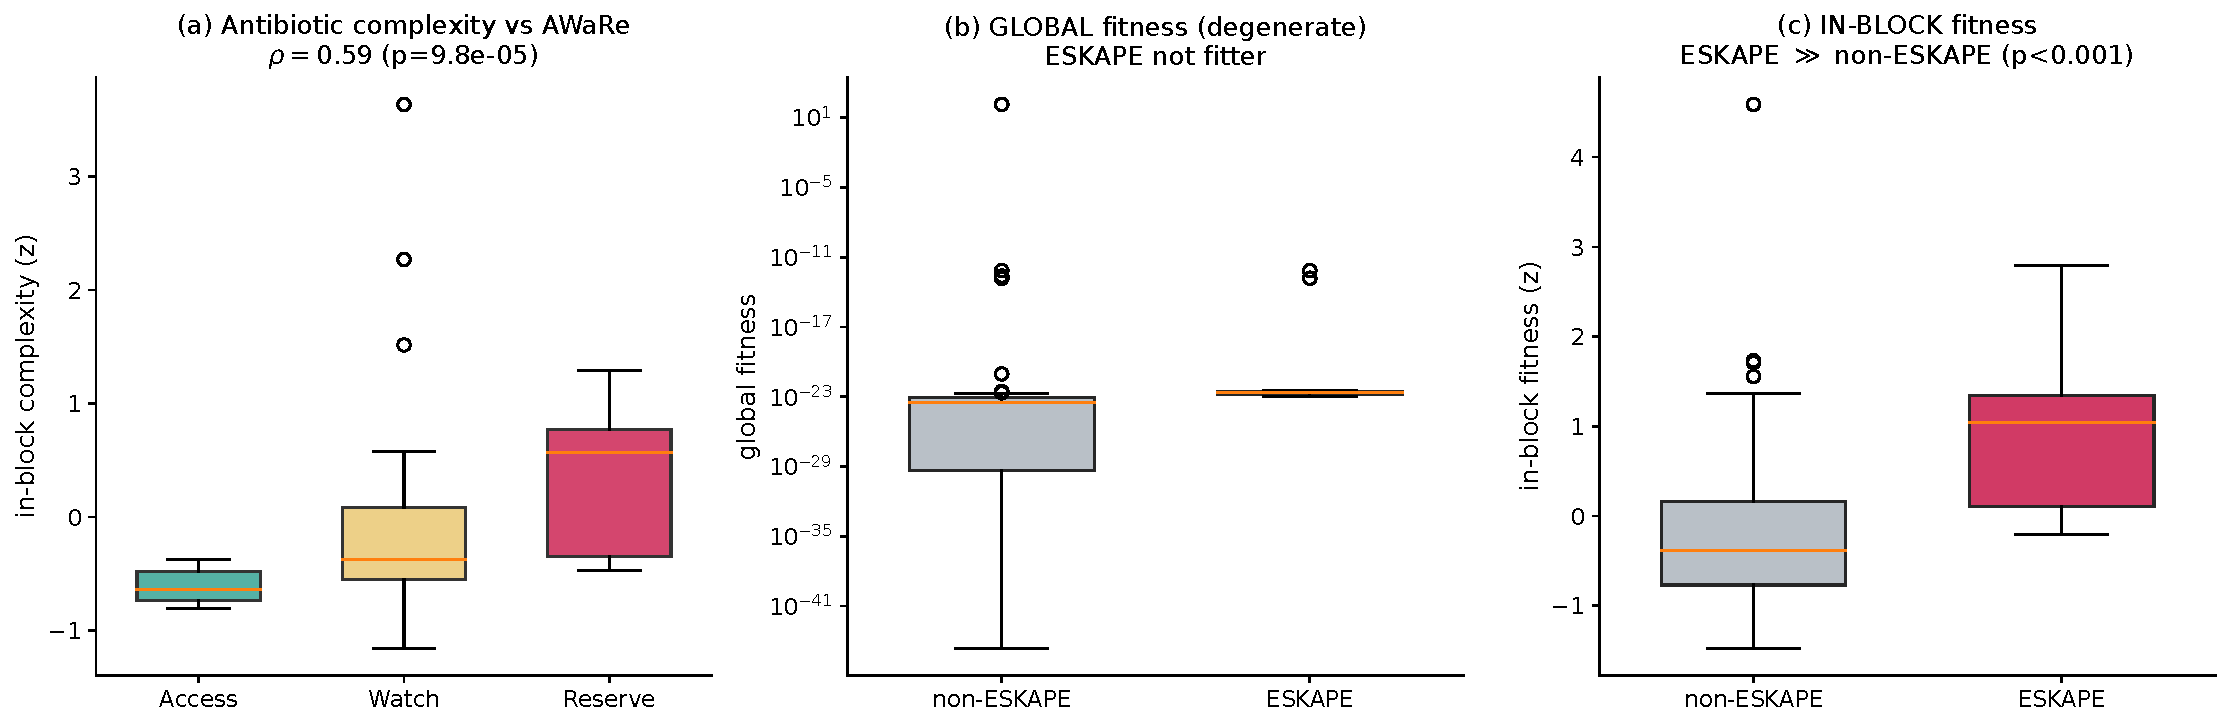
\includegraphics[width=\textwidth]{figures/fig3_efc_validation.pdf}
\caption{\textbf{Fitness and complexity validate against WHO classifications.}
(a) In-block antibiotic complexity increases with the WHO AWaRe tier (Access/Watch/Reserve),
Spearman $\rho=0.6$. (b) \emph{Global} pathogen fitness fails: ESKAPEE organisms are not the fittest
(fitness vs.\ WHO priority $\rho=-0.24$). (c) \emph{In-block} pathogen fitness succeeds: ESKAPEE
organisms are markedly fitter than non-ESKAPEE ($p<10^{-3}$).}
\label{fig:efc}
\end{figure}

\subsection{Predicting where resistance appears next}
The most useful question is whether this structure lets us \emph{anticipate} new resistance. The idea
is that resistances are not independent: drugs that share a mechanism tend to be beaten together. We
make this concrete by building a \emph{co-resistance network} of drugs, linking two antibiotics when
many bugs resist both (Fig.~\ref{fig:pred}a)---its links duly organise by drug family and AWaRe class.
For a species not yet resistant to a drug $a$, we then ask a single question: of the drugs that sit
next to $a$ in this network, how many does the species already beat? This fraction, the
network-exposure score $\rho$, is the same ``adjacent-possible'' logic used to forecast which chess
openings a player will adopt next~\cite{demarzo2023chess}. The bet is that a species surrounded by
drugs it already resists is one short step from resisting $a$ too.

We stress that this predictor has \emph{no free parameters to tune}: both the yes/no cutoff
($\rca\ge1$, the median) and the way the network is built are fixed in advance, so there is nothing
that could be quietly adjusted to flatter the result. This lets us test it in the fairest possible
way---strictly forward in time. For each year we build everything from the past only and predict the
following year's new resistances, repeating this for every year from 2019 to 2023 (predicting
2020--2024); each prediction concerns a future the model has never seen. The score works, and works
consistently. Bugs in the most-exposed group are more than \emph{three times} more likely to acquire the
new resistance than those in the least-exposed group ($17\%$ vs.\ $4.6\%$; Fig.~\ref{fig:pred}b). Its
overall accuracy, measured as the probability of ranking a true future resistance above a non-event
(the AUC), is $0.71$ for the drug network and $0.63$ for the analogous pathogen network (two species
linked when they resist similar drugs), stable across every year tested ($0.67$--$0.77$ and
$0.59$--$0.69$). To be sure this reflects the real wiring and not just how busy each node is, we
reshuffled the network labels \num{200} times: the true score stands far above this chance baseline
($z=6.2$ and $8.7$, $p<0.005$).

The comparison that makes the point is with the obvious na\"ive guesses. Once resistance is measured
by comparative advantage, simply betting on the currently most common resistances, or on the species
that already sit closest to the threshold, predicts nothing at all (AUC $\approx 0.51$, i.e.\ a coin
flip; Fig.~\ref{fig:pred}c). Only the network position carries information. Finally, reading the score
drug by drug flags a shortlist of ``contagion-hub'' antibiotics---ceftazidime, meropenem, gentamicin,
cefepime (Fig.~\ref{fig:pred}d)---whose emerging resistance is the most anticipatable from a species'
existing profile, and which are therefore the natural targets for early warning.

\begin{figure}[t]
\centering
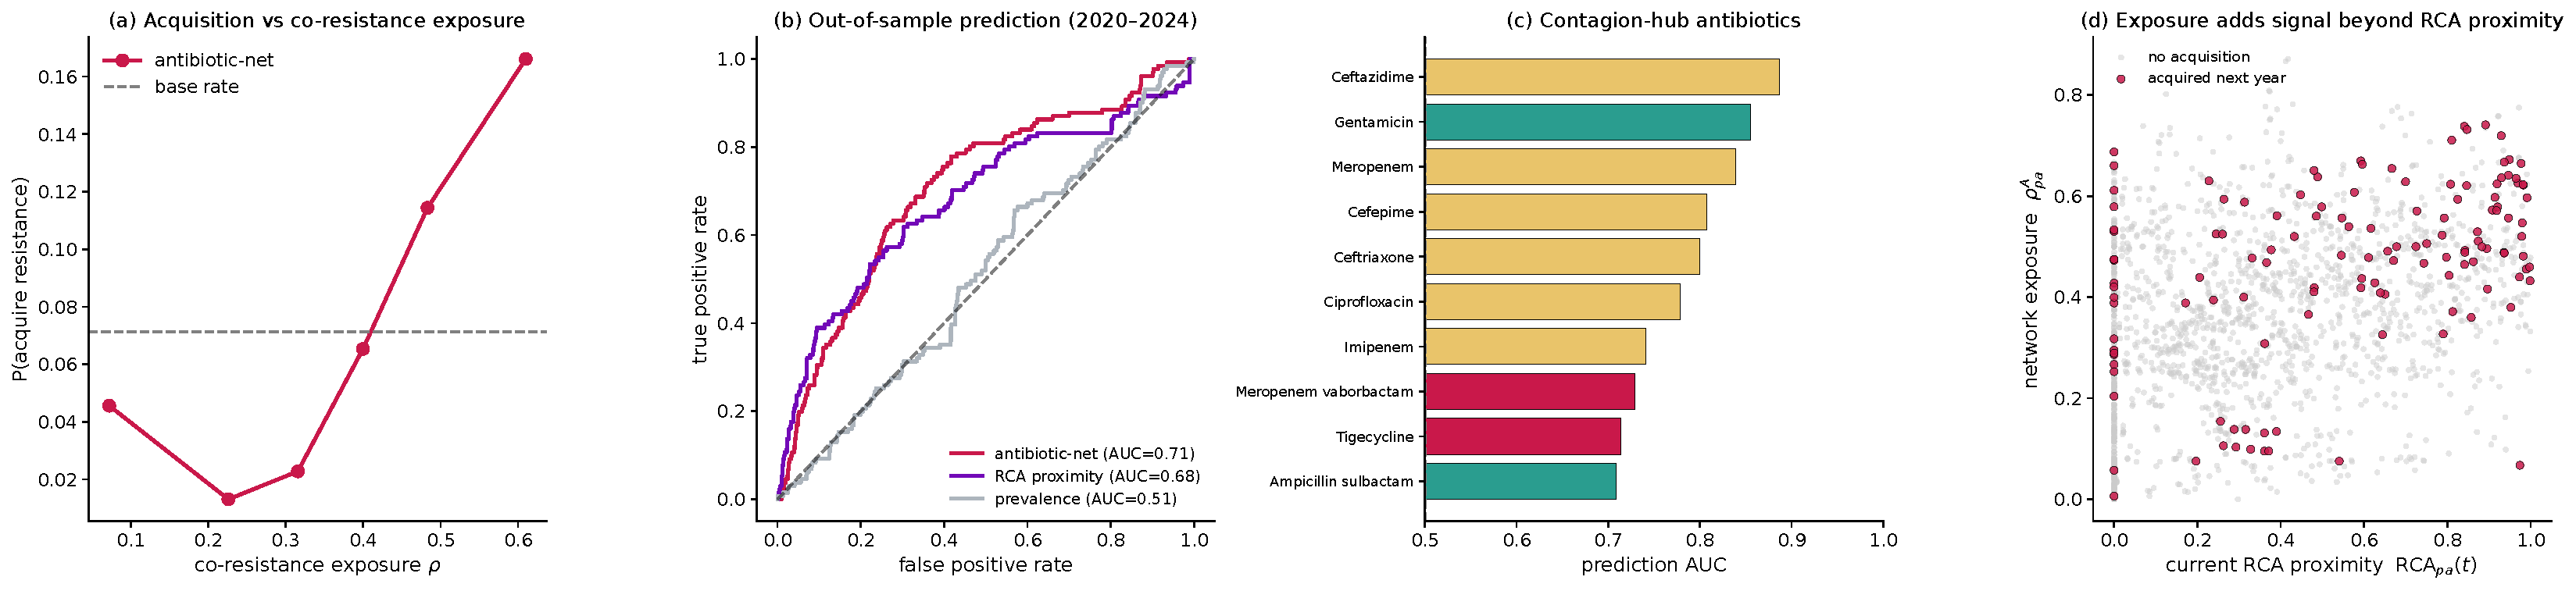
\includegraphics[width=\textwidth]{figures/fig4_prediction.pdf}
\caption{\textbf{Prediction of resistance emergence from network exposure.}
(a) Antibiotic co-resistance network (co-occurrence projection), nodes coloured by WHO AWaRe class, sized by
degree. (b) Probability of acquiring a new resistance versus network-exposure $\rho$ for the antibiotic
and pathogen projections; dashed line is the base rate. (c) Out-of-sample ROC (pooled rolling-origin
test): both network scores beat the prevalence baseline, which is uninformative under RCA. (d)
Contagion-hub antibiotics: per-drug prediction AUC (colour = AWaRe class).}
\label{fig:pred}
\end{figure}

This local-contagion picture can be read directly off the relatedness networks. Fig.~\ref{fig:spread}
follows worked examples over two decades: two pathogens (\textit{Klebsiella pneumoniae},
\textit{Escherichia coli}) progressively light up the antibiotic co-resistance network as they acquire
resistances, and two antibiotics (meropenem, ciprofloxacin) spread across the pathogen relatedness
network as more species become resistant. In every case the newly-lit nodes are network neighbours of
already-lit ones---resistance diffuses through the network rather than appearing at random---which is
exactly the regularity the exposure score exploits.

\begin{figure}[t]
\centering
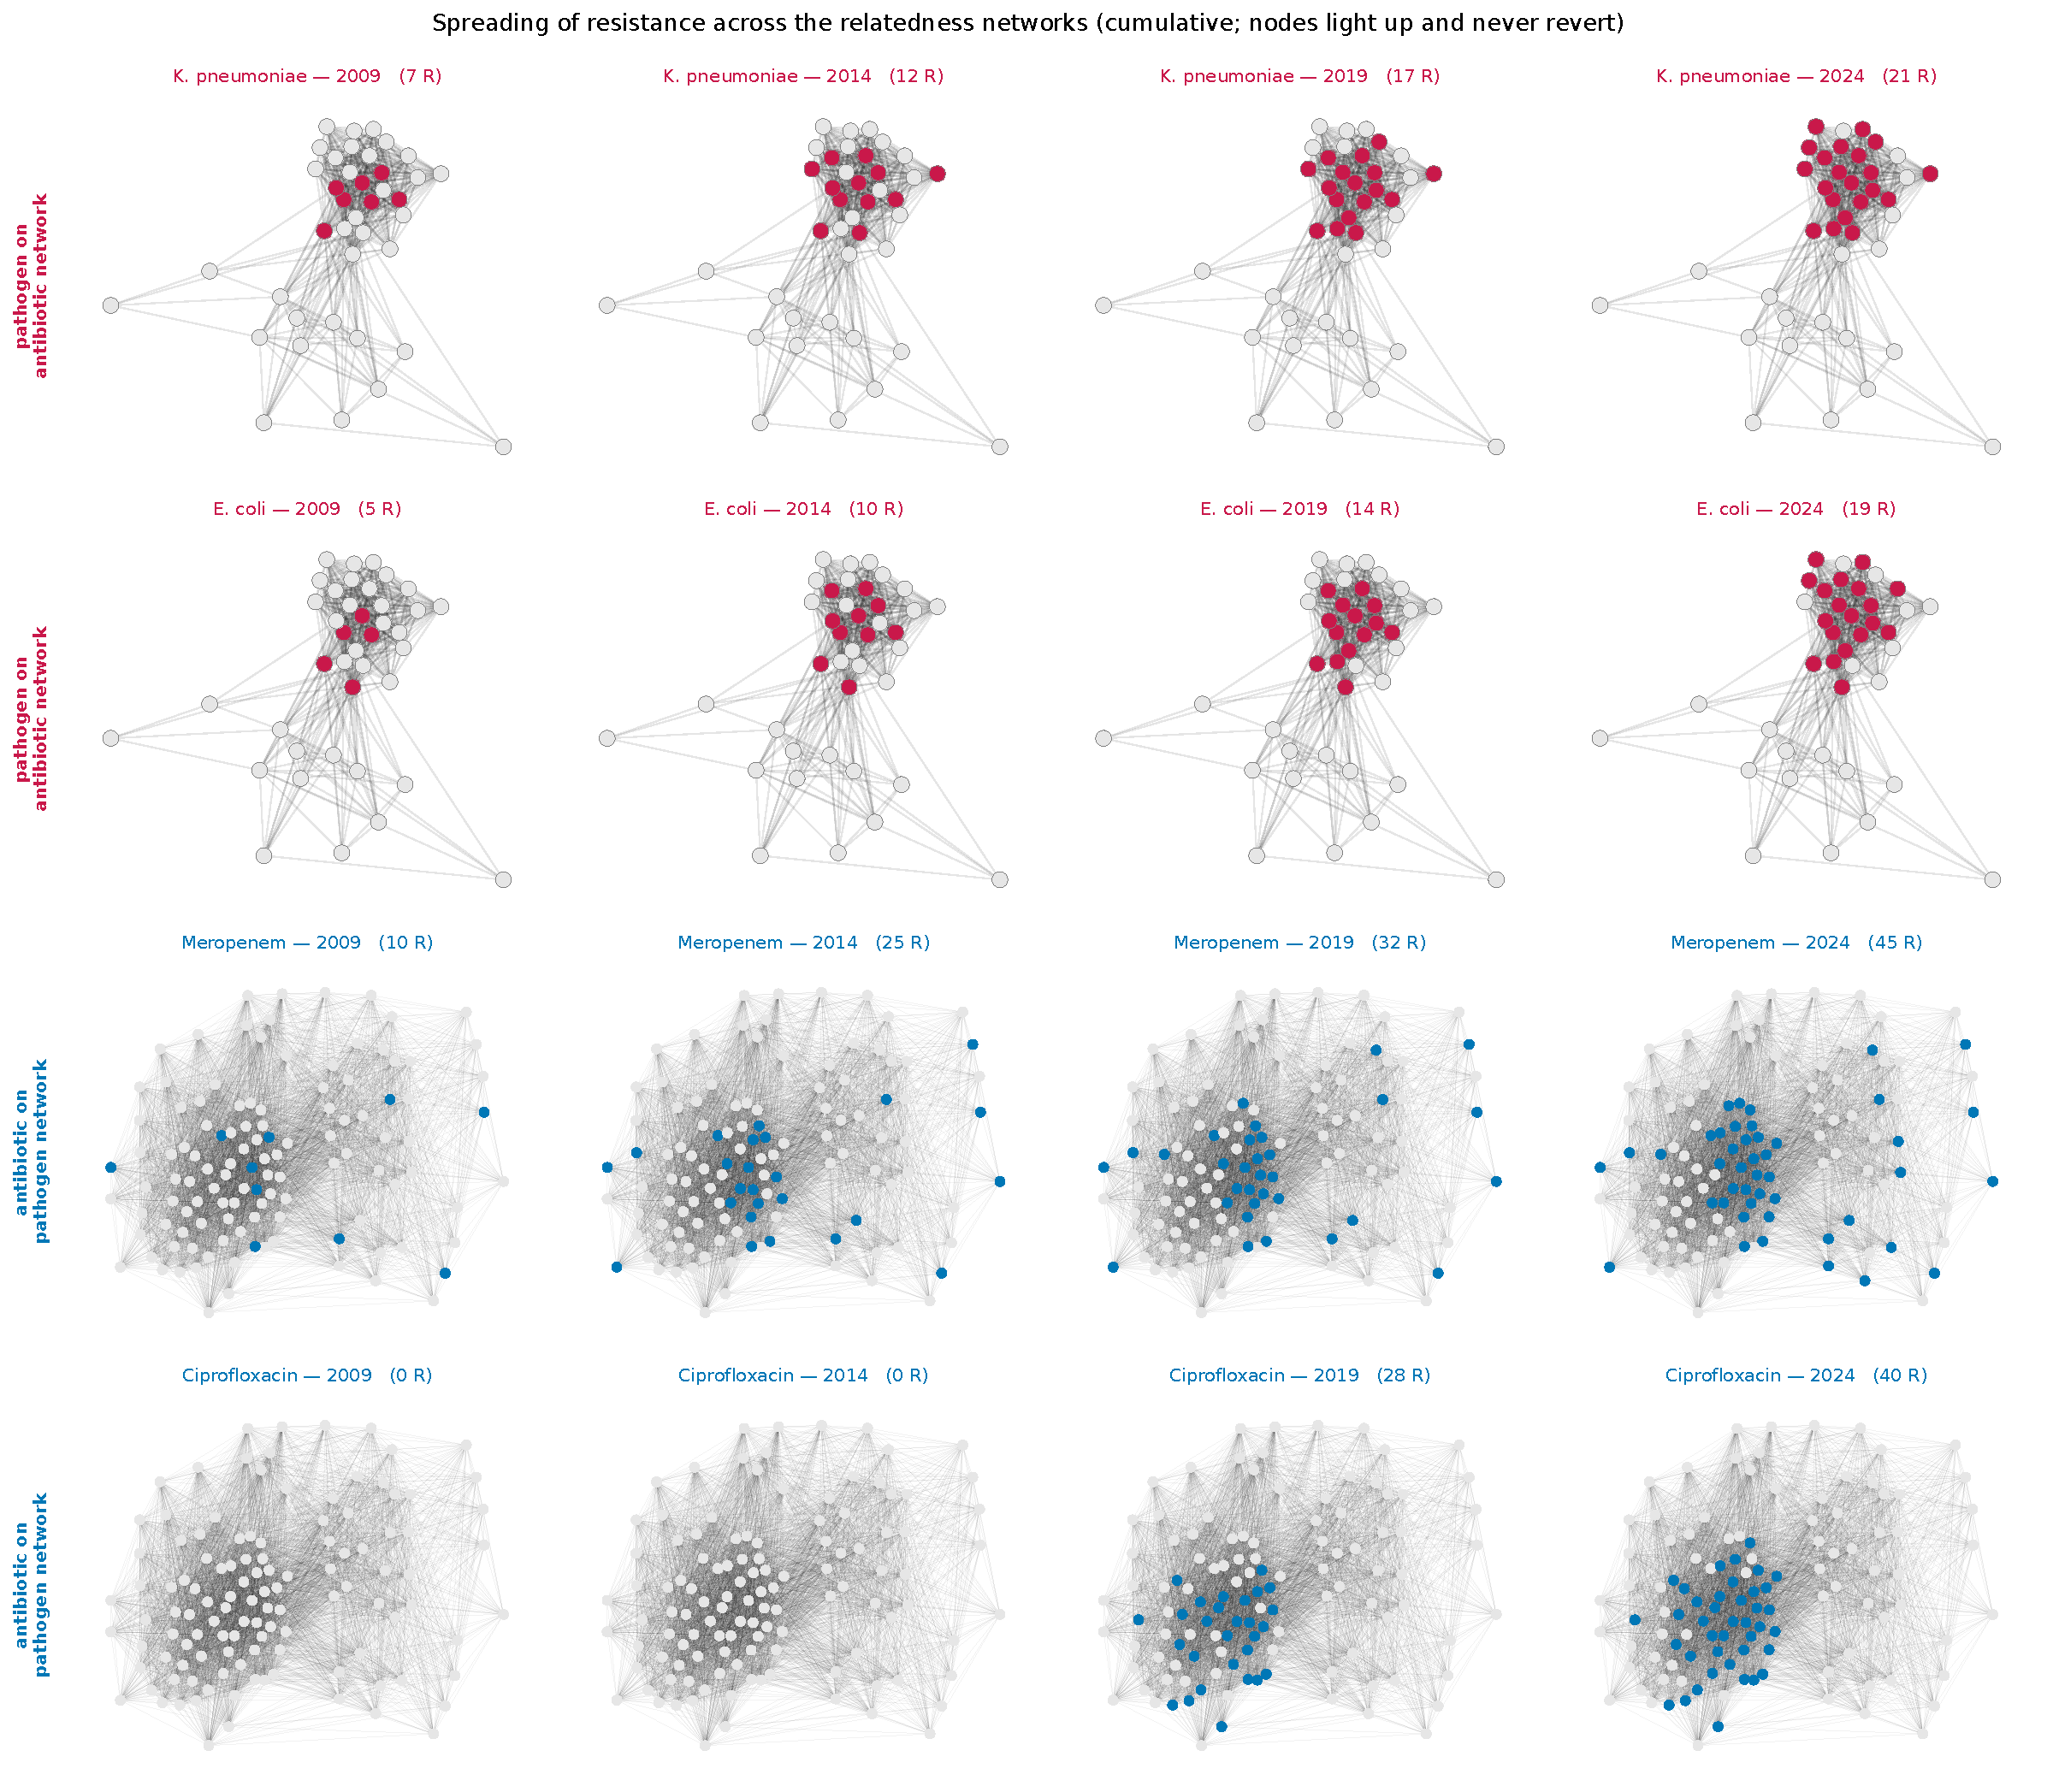
\includegraphics[width=\textwidth]{figures/fig5_spreading.pdf}
\caption{\textbf{Spreading of resistance across the relatedness networks.}
Top two rows: two example pathogens (\textit{K.\ pneumoniae}, \textit{E.\ coli}) shown on the fixed
antibiotic co-resistance network; a node is coloured when the pathogen has acquired RCA-resistance to
that drug by the indicated year (cumulative, so nodes light up and never revert). Bottom two rows: two
example antibiotics (meropenem, ciprofloxacin) shown on the pathogen relatedness network; a node is
coloured when that species has become resistant. Resistance spreads to network-adjacent nodes rather
than at random.}
\label{fig:spread}
\end{figure}

\section{Discussion}
Representing AMR surveillance as a bipartite network and analysing it with Economic Complexity tools
yields a coherent picture that departs from the trade paradigm. AMR is \emph{not} a global complexity
ladder: there is no single axis along which pathogens diversify their resistance and drugs become
progressively harder to overcome. Instead, the network is block-nested---modular by antibiotic
spectrum, with nestedness re-emerging inside each therapeutic ecosystem. This is the same structure
found for firms rather than countries~\cite{laudati2023}, and it has the same methodological
consequence: the Fitness--Complexity algorithm, which presupposes global nestedness, is degenerate
when applied to the whole matrix and must instead be run within the locally-nested blocks. The strong
external validation of the within-block scores against the WHO AWaRe and priority-pathogen
classifications---together with the failure of the global scores---turns this from a technical caveat
into a positive, testable finding.

The practical payoff is prediction. Once resistance is binarized by comparative advantage, neither how
common a resistance is nor how close a pathogen already sits predicts which resistances emerge next;
only network position does. Resistance spreads in the ``adjacent possible'', appearing where a pathogen
is already close, on the co-resistance network, to what it resists---mirroring how chess players adopt
openings adjacent to their repertoire~\cite{demarzo2023chess}. The two projections give complementary
but consistent views, and the per-drug decomposition provides an actionable early-warning list of
antibiotics whose emerging resistance is most anticipatable.

Several limitations temper these conclusions. The predictive AUCs are moderate and rest on a limited
number of acquisition events; genus/species coverage is uneven across the surveillance programme; and
RCA-on-resistance, while natural, is a modelling choice. The blocks are validated against a
degree-preserving null and against expert classifications, but a fully Bayesian bipartite-configuration
treatment and multi-year prediction labels would sharpen the estimates. Nonetheless, the convergence of
structure, validated rankings and out-of-sample prediction suggests that the economic-complexity view
of AMR is both interpretable and useful, and that surveillance data contain exploitable early signals
of where resistance will emerge next.

\section{Methods}

\paragraph{Data.} We use the ATLAS/Vivli antimicrobial susceptibility surveillance programme,
aggregated to species $\times$ antibiotic $\times$ year counts of susceptible/intermediate/resistant
isolates. We retain cells with $N_{\text{tested}}\ge 30$. Unless noted, structural and validation
analyses use the pooled 2015--2024 window (\num{139} pathogens $\times$ \num{40} antibiotics);
prediction uses expanding causal windows (below).

\paragraph{Binarization.} From the pooled resistance fraction $r_{pa}=n^R_{pa}/N_{pa}$ we compute the
revealed comparative advantage
$\rca_{pa} = \big(r_{pa}/\sum_{a'} r_{pa'}\big)\big/\big(\sum_{p'} r_{p'a}/\sum_{p'a'} r_{p'a'}\big)$
and set $M_{pa}=1$ iff $\rca_{pa}\ge 1$, following the standard EC threshold~\cite{laudati2023}. On
these data this threshold coincides with the median of the RCA distribution (median $\rca\in[0.99,1.17]$
across windows), so the binarization is fixed a priori and is not tuned against any outcome.

\paragraph{Nestedness and in-block nestedness.} We use the overlap-based global nestedness $\N$ and
in-block nestedness $\I$ of Refs.~\cite{soleribalta2018,laudati2023}. For row nodes,
$\I \propto \sum_{i,j}\frac{O_{ij}-\langle O_{ij}\rangle}{k_j(C_i-1)}\,\Theta(k_i-k_j)\,\delta(a_i,a_j)$
with an analogous column term, where $O_{ij}$ is the number of shared links,
$\langle O_{ij}\rangle=k_ik_j/N$ the degree-null expectation, $C_i$ the size of $i$'s block and
$\Theta$ the Heaviside function; $\N$ is the single-block case. Blocks are obtained by spectral
co-clustering (we optimise over $k=2\!-\!6$). Significance is assessed against \num{100}
degree-preserving randomisations.

\paragraph{Fitness--Complexity.} We iterate the FC map~\cite{tacchella2012}
$\tilde F_p^{(n)}=\sum_a M_{pa} Q_a^{(n-1)}$, $\tilde Q_a^{(n)}=1/\sum_p M_{pa}/F_p^{(n-1)}$,
normalising each iterate by its mean, to convergence. Global scores use the full matrix; in-block
scores are computed on each block's sub-matrix and $z$-scored within block before pooling.

\paragraph{Projections.} One-mode projections use the plain co-occurrence weighting
$W_{ab}=\sum_p M_{pa}M_{pb}$---the number of species resistant to both drugs $a$ and $b$, symmetric by
construction---for the antibiotic layer, and the analogous $W_{pq}=\sum_a M_{pa}M_{qa}$ for pathogens.
We also verified that a bipartite-configuration (BiCM) validated projection yields essentially no edges,
consistent with co-resistance being degree-explained. Among the projection weightings we tried, this
raw co-occurrence gave the best out-of-sample prediction: degree-normalised weightings consistently
\emph{lowered} the AUC (e.g.\ $0.71\to0.67$ under a symmetric degree normalisation), because the common,
widely-shared co-resistances they down-weight are exactly what carries the predictive signal here.

\paragraph{Network-exposure prediction.} The predictor is deliberately parameter-free, so that no
quantity is tuned against the test set: the binarization ($\rca\ge 1$, the distribution median) and the
projection (plain co-occurrence) are both fixed a priori, and the exposure score is a pure ranking. For each origin
year $t$ we build $M$, the projection $W$ and each pathogen's repertoire from data with year $\le t$,
and define the exposure $\rho_{pa}=\sum_{o} W_{ao} M_{po}/\sum_o W_{ao}$. Candidates are $(p,a)$ pairs
susceptible and observed at $t$ and observed at $t+1$; the label is $\rca$-resistance at $t+1$. Because
there is nothing to fit, we evaluate by \emph{rolling origin}: every origin $t=2019\ldots2023$
(predicting $2020\ldots2024$) is a genuine out-of-sample test, and we report the rank-based AUC per
origin and pooled. Significance uses \num{200} permutations of the network node labels. Baselines are
resistance prevalence and current proximity-to-threshold. A separate robustness sweep over alternative
binarizations (absolute thresholds, $\rca\ge1.5$) and projection weightings (degree-normalised,
BiCM-validated) confirms that the plain co-occurrence choice is the simplest available and is not
optimised against the test set---if anything the alternatives we tried predicted less well.

\paragraph{External validation.} Antibiotic complexity is compared (Spearman) to the WHO AWaRe class
(Access/Watch/Reserve), taken from the WHO 2023 AWaRe classification~\cite{who_aware} (all
\num{43} antibiotics mapped; see the reference table shipped with the data). Pathogen fitness is
compared to the WHO bacterial-priority tier and to ESKAPEE membership (the ESKAPE priority pathogens
plus \textit{E.\ coli}; Mann--Whitney).

\begin{thebibliography}{9}
\bibitem{hidalgo2009} C. A. Hidalgo and R. Hausmann, \textit{PNAS} \textbf{106}, 10570 (2009).
\bibitem{tacchella2012} A. Tacchella \textit{et al.}, \textit{Sci. Rep.} \textbf{2}, 723 (2012).
\bibitem{aufiero2024} S. Aufiero, G. De Marzo \textit{et al.}, \textit{Sci. Rep.} \textbf{14}, 11752 (2024).
\bibitem{demarzo2023chess} G. De Marzo and V. D. P. Servedio, \textit{Sci. Rep.} \textbf{13}, 5327 (2023).
\bibitem{laudati2023} D. Laudati, M. S. Mariani, L. Pietronero, A. Zaccaria, \textit{J. Phys. Complex.} \textbf{4}, 025011 (2023).
\bibitem{soleribalta2018} A. Sol\'e-Ribalta \textit{et al.}, \textit{Phys. Rev. E} \textbf{97}, 062302 (2018).
\bibitem{who_aware} World Health Organization, \textit{AWaRe classification of antibiotics for evaluation and monitoring of use, 2023} (WHO/MHP/HPS/EML/2023.04, Geneva, 2023).
\bibitem{murray2022} C. J. L. Murray \textit{et al.}, \textit{Lancet} \textbf{399}, 629 (2022).
\end{thebibliography}

\end{document}
